\begin{figure}[htbp]
  \centering
  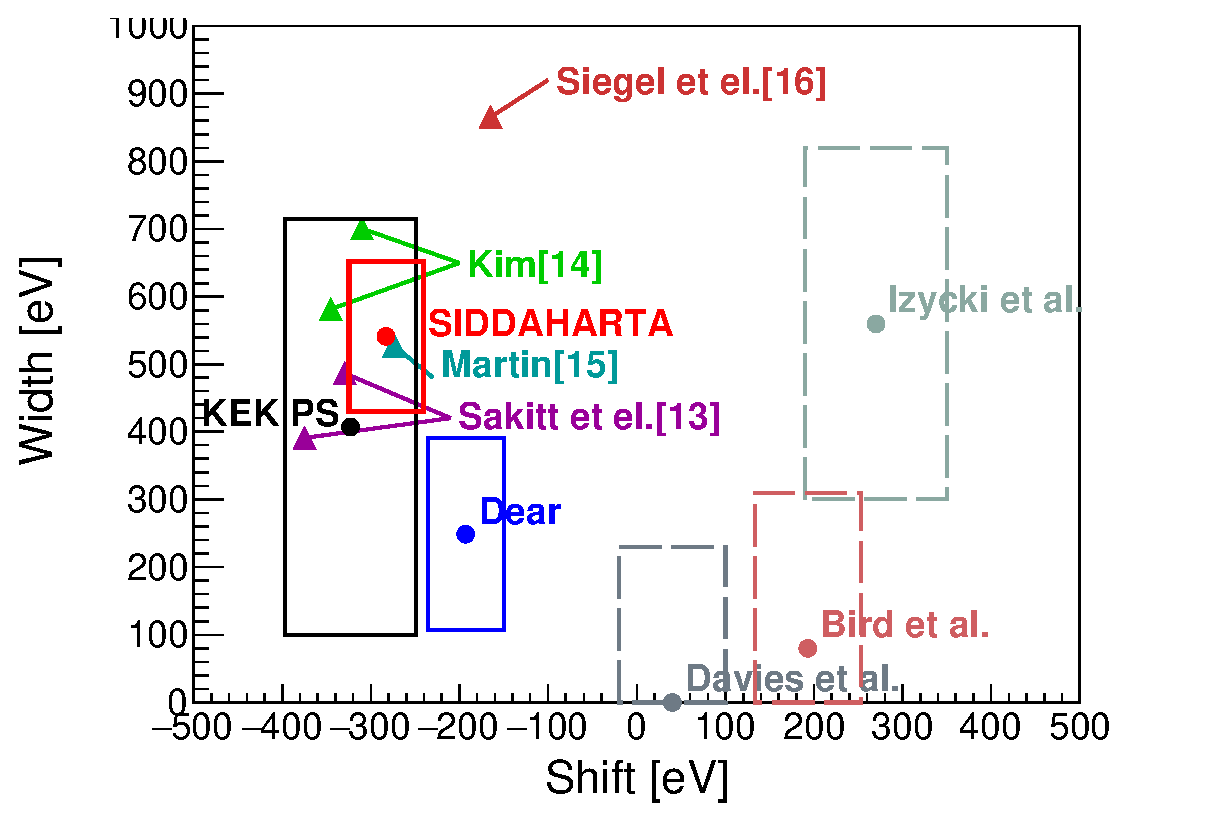
\includegraphics[width=12cm]{../pic/Dron/KN_int_map.eps}
  \caption{
    This figure is shown about the kaonic hydrogen.
    Triangle markers indicate theoretical calculations where $\bar{K}N$ scattering data were extrapolated to the $\bar{K}N$ threshold.
    Circle markers represent experimental values, and error ranges in the energy shift and width are indicated by squares.
    Dashed lines correspond to experiments using hydrogen gas targets conducted prior to 1990,
    while solid lines represent experiments conducted afterward.
  }
  \label{fig:KN_int}
\end{figure}
